%!TEX root = ../main.tex
\begin{frame}{\emph{Smart} TVs}
   \ \  \\[0.1cm]
  \begin{itemize}
  \item Capacidades interativas
  \item Conexão à internet
  \item Conteúdo de mídia transmitido a partir de outros dispostivo
\end{itemize}
\end{frame}

\begin{frame}{\emph{Smart} TVs}
\begin{figure}[h!]
	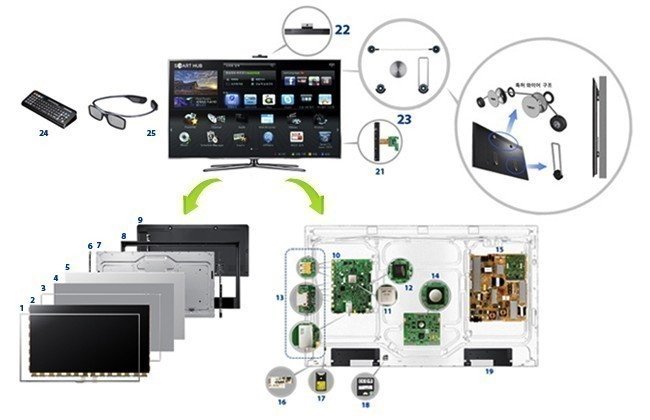
\includegraphics[width=\textwidth]{img/smart_samsung.jpg}
	\caption{Diagrama representativo de uma \emph{Smart} TV e seus componentes}
	\label{fig:smart_samsung}
\end{figure}
\end{frame}


\begin{frame}{\emph{Smart} TVs}
  \begin{figure}[h!]
  	\centering
  	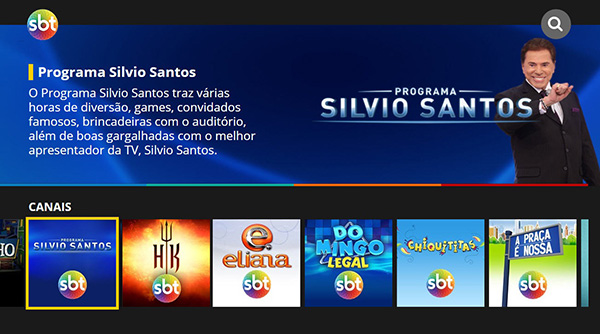
\includegraphics[width=\textwidth]{img/sbt_app.jpg}
  	\caption{Aplicativo SBT}
  	\label{fig:sbt_app}
  \end{figure}
\end{frame}

\begin{frame}{\emph{Smart} TVs}
   \ \  \\[0.1cm]
  \begin{itemize}
  \item PNAD 2015
  \begin{itemize}
    \item $103$ milhões de aparelhos de televisões em residências e pontos comerciais
    \item $16$ milhões de \emph{Smart} TVs
    \item $94\%$ destas \emph{Smart} TVs foram adquiridas entre $2014$ e $2015$
    \item $68,2\%$ do total de televisores vendidos no primeiro semestre de $2017$
  \end{itemize}
\end{itemize}
\end{frame}

\begin{frame}{\emph{Smart} TVs}
   \ \  \\[0.1cm]
  \begin{itemize}
  \item Benefícios resultantes do uso de \emph{Smart}

  \item Encerramento da transmissão de sinal analógico da televisão aberta
  \item Copa do Mundo 2018
  \item Tecnologia 4K
\end{itemize}
\end{frame}

\begin{frame}{Classificação Indicativa}
   \ \  \\[0.1cm]
  \begin{itemize}
  \item Sistema de garantias dos direitos da criança e do adolescente
  \item Reserva-se o direito final aos pais e responsáveis
  \item Órgão responsável: Cocind, vinculada ao Ministério da Justiça
  \item Análise de classificação indicativa
  \begin{itemize}
    \item Grau de incidência de conteúdos impróprios
  \end{itemize}
\end{itemize}
\end{frame}

\begin{frame}{Machine Learning}
   \ \  \\[0.1cm]
  \begin{itemize}
  \item Estudo sistemático de algoritmos e sistemas que são capazes de melhorar seu desempenho com a experiência
  \item Modelo ou função que mapeie as instâncias do espaço de entrada para o de saída
  \item Paradigmas de Aprendizado
  \begin{itemize}
    \item Aprendizado Supervisionado
    \item Aprendizado Não-Supervisionado
    \item Aprendizado por Reforço
  \end{itemize}
  \item Tarefas de Aprendizado
  \begin{itemize}
    \item Classificação
    \item Regressão
  \end{itemize}
\end{itemize}
\end{frame}

\begin{frame}{Redes Neurais Artificiais}
   \ \  \\[0.1cm]
  \begin{itemize}
  \item Cérebro humano
  \item Neurônios: unidades de processamento simples
  \item Capacidade de capturar tendências
  \item Generalização
\end{itemize}
\end{frame}

\begin{frame}{Redes Neurais Artificiais}
   \ \  \\[0.1cm]
  \begin{itemize}
  \item McCulloch e Pitts
  \begin{figure}[ht]
  	\centering
  	\caption{Representação de um neurônio artificial}
  	\label{fig:neuronio}
  	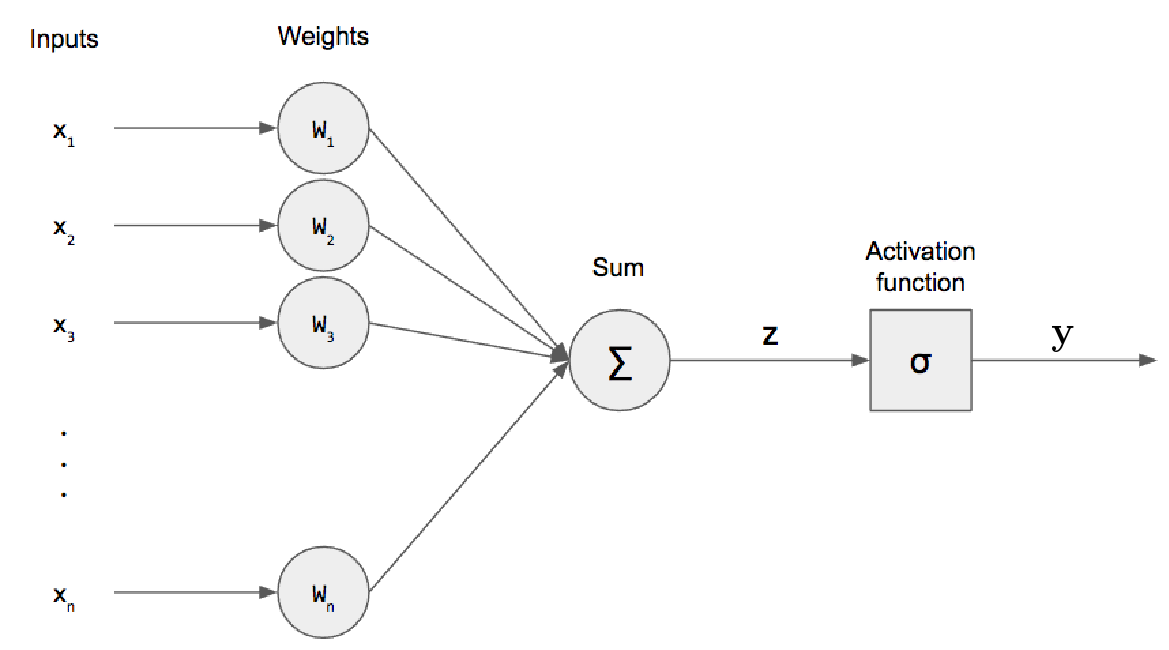
\includegraphics[width=0.7\textwidth]{img/perceptron.png}
  \end{figure}
\end{itemize}
\end{frame}

\begin{frame}{Redes Neurais Artificiais}
   \ \  \\[0.1cm]
  \begin{itemize}
  \item Perceptron de Rosenblatt (1958)
  \begin{itemize}
    \item Algoritmo de aprendizado
    \item Endereçar apenas problemas linearmente separáveis
  \end{itemize}
\end{itemize}
\end{frame}

\begin{frame}{Redes Neurais Artificiais}
   \ \  \\[0.1cm]
   \begin{figure}[!h]
   	\caption{Arquiteturas populares de RNAs.}
   	\label{fig:popular_archs}
   	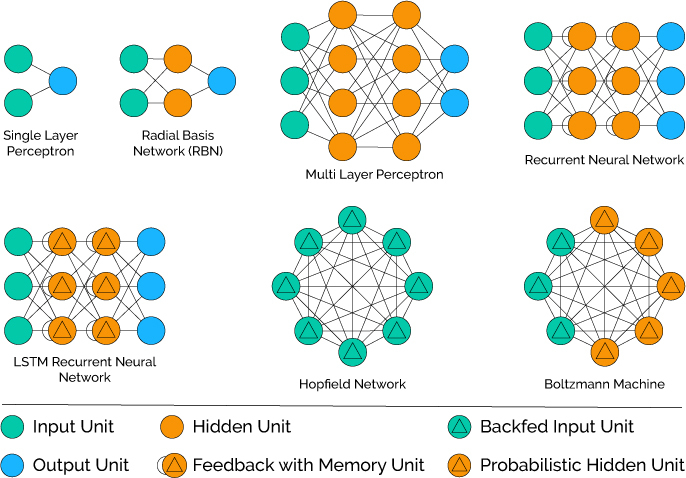
\includegraphics[width=\linewidth]{img/popular_archs}
   \end{figure}
\end{frame}

\begin{frame}{Redes Neurais Artificiais}
   \ \  \\[0.1cm]
   %!TEX root = ../sbc-template.tex

\begin{table}[ht]
	\scalefont{0.8}
	\centering
	\caption{Funçoes de ativação mais populares. ---melhorar legenda}
	\label{tab:ativacoes}
	\begin{tabular}{l l p{6.5cm} l}
		\toprule
		Nome 			 		& Gráfico & Equação & Intervalo\\
		\midrule
		Identidade ou Linear		&
		 	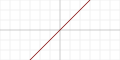
\includegraphics[width=0.1\textwidth]{img/identidade.png}
			&
			$
				\begin{aligned}
					g(z) = z
				\end{aligned}
			$
			& $(-\infty, + \infty) $\\
		\hline
		Tangente Hiperbólica		&
			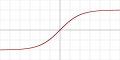
\includegraphics[width=0.1\textwidth]{img/tanh.png}
			&
			$
				\begin{aligned}
					g(z) = tanh(z) =\frac{(e^z - e^{-z})}{(e^z + e^{-z})}
				\end{aligned}
			$
			 & $(-1,1)$\\
		\hline
		Sigmoide ou Logística		&
			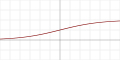
\includegraphics[width=0.1\textwidth]{img/sigmoid.png}
			&
			$
				\begin{aligned}
					g(z) = \sigma(z) = \frac{1}{1+e^{-x}}
				\end{aligned}
			$
			& $ (0,1) $\\
		\hline
		Unidade Linear Retificada	&
			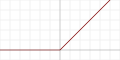
\includegraphics[width=0.1\textwidth]{img/relu.png}
			&
			$
				\begin{aligned}
					g(z) = max(0,z)
				\end{aligned}
			$
			& $ [0, \infty) $\\
		\hline
		Softmax					&
			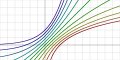
\includegraphics[width=0.1\textwidth]{img/softmax.png}
			&
			$
				\begin{aligned}
					g(\alpha, z) =
						\begin{cases}
							-\frac{ln(1-\alpha(z+\alpha))}{\alpha}, & \text{se } \alpha < 0\\
							z, & \text{se } \alpha = 0 \\
							\frac{e^{\alpha z} -1}{\alpha} + \alpha, & \text{se } \alpha > 0
						\end{cases}
				\end{aligned}
			$
			& $(-\infty, \infty)$\\
		\bottomrule
	\end{tabular}
\end{table}

\end{frame}

\begin{frame}{Redes Neurais Artificiais}
   \ \  \\[0.1cm]
   \begin{itemize}
     \item Hiperparâmetros de uma RNA
     \begin{itemize}
       \item Taxa de aprendizado
       \item Funções de ativação
       \item Arquitetura da rede
       \item \emph{batch size}
       \item Número de épocas
     \end{itemize}
   \end{itemize}
\end{frame}

\begin{frame}{Redes Neurais Artificiais}
   \ \  \\[0.1cm]
  \begin{itemize}
  \item Algoritmo de treinamento de uma RNA
  \item Entrada: Conjuntos de exemplos e respectivos rótulos $(X,Y)$, rede neural a ser treinada, número de épocas $e$, taxa de aprendizado $\eta$ e \emph{batch size} $b$.
  \item Saida: Rede neural treinada.
  \begin{enumerate}

    \item Inicialização dos vetores de pesos $w$ e \emph{bias} $b$
    \item Para cada \emph{batch} = 1,\ldots, b do conjunto de dados:
    \begin{enumerate}
      \item Fase \emph{forward}: Calcular previsões $\hat{y}$ e custos $J$.
      \item Fase \emph{backwards}: Calcular gradientes dos pesos $\nabla_{w^c}$ e \emph{bias} $\nabla_{b^c}$
      \item Atualizar valores dos pesos e \emph{bias} a partir do gradiente descendente.
    \end{enumerate}
  \end{enumerate}
\end{itemize}
\end{frame}

\begin{frame}{Deep Learning}
   \ \  \\[0.1cm]
   \begin{itemize}
     \item Capacidade de representar e reconhecer características sucessivamente complexas
     \item Adição de níveis ou camadas de operações não-lineares
     \item Resolver problemas complexos com um desempenho cada vez maior
     \begin{itemize}
       \item Aumento recente da quantidade de dados disponíveis sobre temas complexos
       \item Aumento da disponibilidade de recursos computacionais para executar modelos mais robustos
     \end{itemize}
   \end{itemize}
\end{frame}

\begin{frame}{Deep Learning}
   \ \  \\[0.1cm]
   \begin{figure}[ht]
   	\centering
   	\caption{Evolução de profunidade, taxa de erro e número de parâmetros das redes neurais profundas com o passar dos anos.}
   	\label{fig:compara_redes}
   	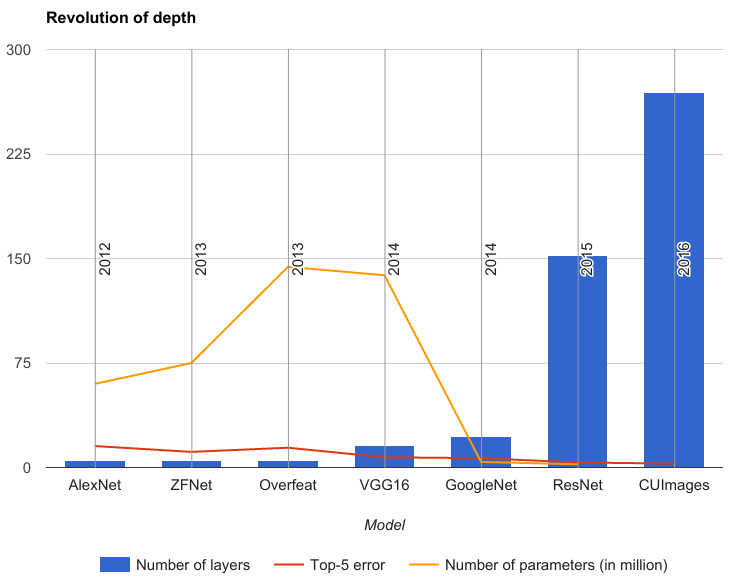
\includegraphics[width=0.8\textwidth]{img/compara_redes.png}
   \end{figure}
\end{frame}

\begin{frame}{Deep Learning}
   \ \  \\[0.1cm]
   \begin{itemize}
     \item Breve Histórico
     \begin{itemize}
       \item (1950) Proposição de modelos lineares simples: McCulloch e Pitts; Perceptron
       \item (1980) Interconexão entre vários neurônios e a proposição do algoritmo \emph{back-propagation} para ajuste de pesos no treinamento das RNAs
       \begin{itemize}
         \item LeNet
       \end{itemize}
       \item (2006) Modelos compostos de várias camadas sucessivas de operações não lineares utilizados para o aprendizado de determinada tarefa
     \end{itemize}
   \end{itemize}
\end{frame}

\begin{frame}{Deep Learning}
   \ \  \\[0.1cm]
   \begin{itemize}
     \item \emph{ImageNet Large Scale Visual Recognition Challenge} (ILSVRC)
     \begin{itemize}
       \item Imagenet
       \item $14$ milhões de imagens de $21$ mil categorias organizadas hierarquicamente
       \item Erro top-5
     \end{itemize}
   \end{itemize}
\end{frame}

\begin{frame}{Deep Learning}
   \ \  \\[0.1cm]
   \begin{figure}[ht]
   	\centering
   	\caption{Evolução do erro dos modelos vencedores da competição ILSVRC pela profundidade das redes neurais}
   	\label{fig:compara_redes_ilsvrc}
   	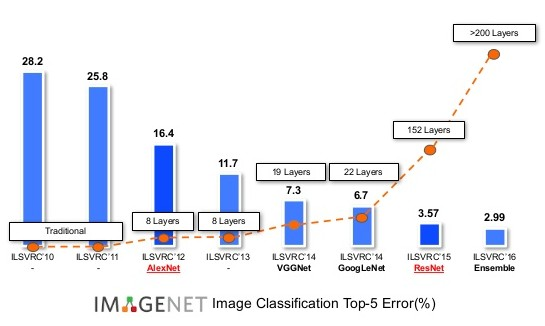
\includegraphics[width=0.8\textwidth]{img/compara_redes_ilsvrc.png}
   \end{figure}
\end{frame}

\begin{frame}{Redes Neurais Convolucionais}
   \ \  \\[0.1cm]
   \begin{itemize}
     \item Topologia bem definida e estrutura em grade
     \item Operações de convolução em pelo menos uma de suas camadas
     \item Destaca-se no reconhecimento de padrões em dados de alta dimensionalidade
   \end{itemize}
\end{frame}

\begin{frame}{Redes Neurais Convolucionais}
   \ \  \\[0.1cm]
   \begin{itemize}
     \item Convolução
     \begin{equation}
      S(i,j) = I(i,j)*K(i,j) = \sum_{m}\sum_{n}I(m,n)K(i-m,j-n)\label{eq:conv_img}
     \end{equation}
   \end{itemize}
   \begin{figure}[!h]
   	\centering
   	\caption{Papel das camadas convolucionais e \emph{feature maps} nas CNNs.}
   	\label{fig:convolutions}
   	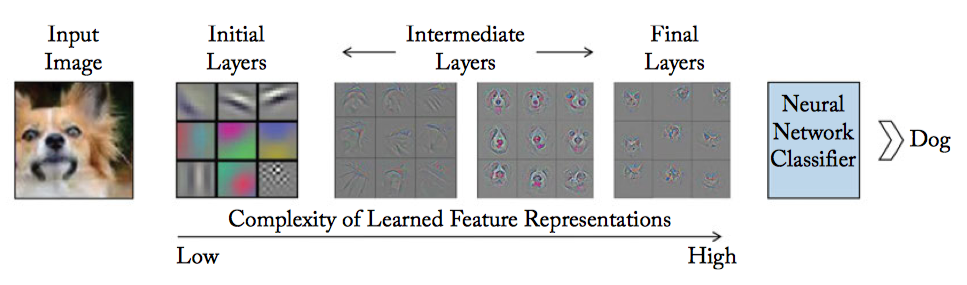
\includegraphics[width=0.8\textwidth]{./img/fundamenta/convolutions}
   \end{figure}
\end{frame}

\begin{frame}{Redes Neurais Convolucionais}
   \ \  \\[0.1cm]
   \begin{figure}
   	\centering
   	\caption{Componentes de uma camada de uma rede neural convolucional.}
   	\label{fig:cnn_camada}
   	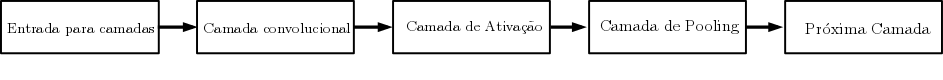
\includegraphics[width=\textwidth]{img/cnn_camada_ipe.png}
   \end{figure}
\end{frame}

\begin{frame}{Redes Neurais Convolucionais}
   \ \  \\[0.1cm]
   \begin{itemize}
     \item Hiperparâmetros de uma CNN
     \begin{itemize}
       \item Pooling
       \item Padding
       \item Strides
     \end{itemize}
   \end{itemize}
\end{frame}

\begin{frame}{Modelos Canônicos de Redes Neurais Convolucionais}
   \ \  \\[0.1cm]
   \begin{itemize}
     \item Arquiteturas que trouxeram contribuições importantes
     \item Comuns ainda hoje no cenário de DL
   \end{itemize}
\end{frame}

\begin{frame}{Modelos Canônicos de Redes Neurais Convolucionais}
   \ \  \\[0.1cm]
   \begin{itemize}
     \item LeNet (1998)
     \begin{itemize}
       \item Conjunto de dados \emph{Modified National Institute of Standards and Technology} (MNIST)
       \item Imagens em escala de cinza de tamanho $32 \times 32$
       \item Amplamente utilizada por bancos
     \end{itemize}
     IMAGEM DA LENET
   \end{itemize}
\end{frame}

\begin{frame}{Modelos Canônicos de Redes Neurais Convolucionais}
   \ \  \\[0.1cm]
   \begin{itemize}
     \item AlexNet (2012)
     \begin{itemize}
       \item Primeira CNN ganhadora do desafio ILSVRC
       \item Imagens de 1000 categorias da ImageNet
       \item Erro top-5 igual a $15.4\%$
       \item Treinamento: duas GPU GTX 580 por 5 a 6 dias
     \end{itemize}
     IMAGEM DA AlexNet
   \end{itemize}
\end{frame}

\begin{frame}{Modelos Canônicos de Redes Neurais Convolucionais}
   \ \  \\[0.1cm]
   \begin{itemize}
     \item VGG (2014)
     \begin{itemize}
       \item Erro top-5 de $7.3\%$
       \item Treinamento em 4 GPUs Nvidia Titan Black por duas a três semanas
       \item Erro top-5 igual a $15.4\%$
     \end{itemize}
     IMAGEM DA VGG
   \end{itemize}
\end{frame}

\begin{frame}{Modelos Canônicos de Redes Neurais Convolucionais}
   \ \  \\[0.1cm]
   \begin{itemize}
     \item Inception ou GoogLeNet (2014)
     \begin{itemize}
       \item 22 camadas convolucionais
       \item Treinamento em algumas GPUs de alta performance por uma semana
       \item Erro top-5 de $6.7\%$
     \end{itemize}
     \begin{figure}[h!]
     	\centering
     	\caption{Bloco Inception da CNN GoogLeNet}
     	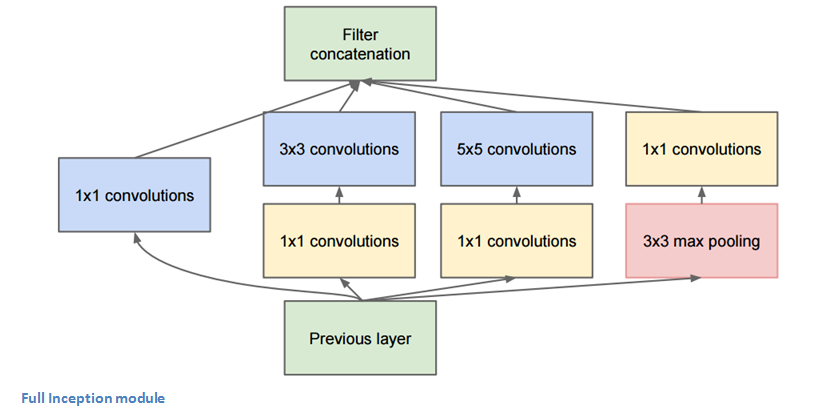
\includegraphics[width=0.7\linewidth]{img/GoogLeNet}
     	\label{fig:bloco_inception}
     \end{figure}
   \end{itemize}
\end{frame}

\begin{frame}{Modelos Canônicos de Redes Neurais Convolucionais}
   \ \  \\[0.1cm]
   \begin{itemize}
     \item ResNet (2015)
     \begin{itemize}
       \item Total de 152 camadas
       \item Treinamento em 8 GPUs por duas a três semanas
       \item Erro top-5 de $3.6\%$
     \end{itemize}
     \begin{figure}[h!]
     \centering
     \caption{Bloco Residual da CNN ResNet.}\label{fig:bloco_residual}
     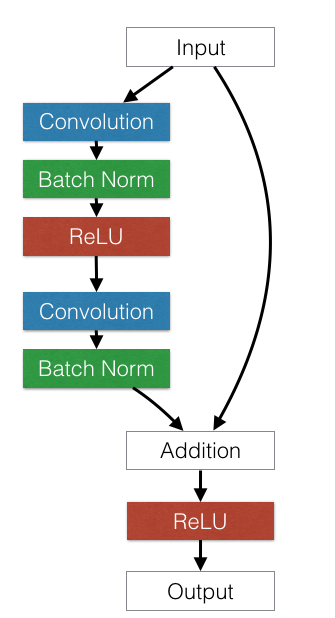
\includegraphics[height=0.3\textheight]{img/resnets_modelvariants}
     \end{figure}
   \end{itemize}
\end{frame}

\begin{frame}{Transfer Learning}
   \ \  \\[0.1cm]
   \begin{itemize}
     \item CNNs com alto desempenho
     \item COLOCAR UM BLOCK
     \item Representações de imagens aprendidas por CNNs a partir de conjuntos de dados com grande número de exemplos podem ser transferidas eficientemente para outras tarefas de reconhecimento visual que tenham uma quantidade limitada de dados de treinamento
     \item Transferir os parâmetros de peso $w$ e de bias $b$
     \item Remove-se as últimas camadas
   \end{itemize}
\end{frame}
